% arara: xelatex: { shell: yes }
% arara: biber
% arara: nomencl
% arara: xelatex: { shell: yes }
% arara: xelatex: { shell: yes }
\documentclass[english]{ttlab-qualify}
% mögliche Optionen:
% - ngerman
% - english
% - minted
% - algorithm
% - nomencl
% - nolibertine

\usepackage{tikz}  

\begin{document}
\titlehead{
  \textbf{Goethe University}\\
  \textbf{Institute for Informatics}\\
  \textbf{Databases and Information Systems (DBIS)}
}
\subject{Bachelor Thesis}
\author{Nils Dambowy}
\title{Topic Models}
\subtitle{Untertitel}
\date{24.12.2022}
\publishers{Supervised by \\ Dr. Karsten Tolle\\ Sebastian Grampe}

\maketitle
\tableofcontents

\chapter{Introduction}    
\section{Problem description}
\section{Thesis structure}

\chapter{Corpus Nummorum and the D4N4}
\section{Corpus Nummorum}
The Corpus Nummorum \textbf{(CN)} is a  research database, which is  the result of the joint work of the Münzkabinett Berlin, Berlin-Brandenburg Academy of Sciences and Humanities (BBAW) and the Big Data Lab of Goethe University, with the motivation to offer ancient Greek coinage for research purposes.\footnote{https://www.corpus-nummorum.eu/about}
It contains information about coins with origin in the regions of Lower Moesia, Thrace, Mysia, and the Troad. Added together, the database contains information about approx. 27,500 coins, 14,000 coming from the area of Thrace and 14,500 from the remaining regions. It is also possible to contribute coins to the database yourself.

\begin{figure}[!htb]%
    \centering%
    \begin{minipage}{.5\textwidth}%
        \centering%
        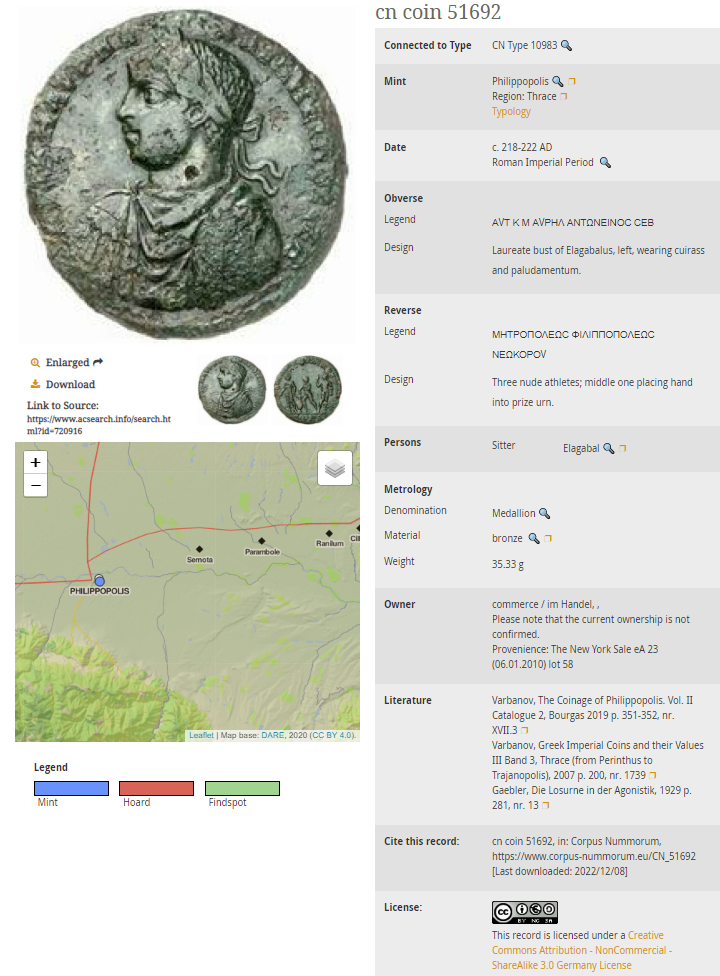
\includegraphics[scale=0.4]{coin_example.png}\\
        \textbf{An example of a coin in the database}\footnotemark[2]%
        \label{fig:coin_example}%
    \end{minipage}%
    \begin{minipage}{0.5\textwidth}%
       All of this information is accessible through the  CN Online Website by using the provided search tool, which lets you filter coins by e.g. epoch, tribe, weight or material. Beside the mentioned characteristics, the CN offers text descriptions of the depicted images on the front- and back side of the coins. To allow a better comparison between different coins, all properties have to be entered in accord to a standardized scheme.\footnotemark[3]  This not only guarantees the previous mentioned upsides but also make entering coins more accessible since e.g. volunteers do not have to worry about having to come up with a scheme themselves. The scheme offers guidelines on how to describe the obverse and reverse of the coin, figures or architecture, portraits, scenes or some general information on how properly describe a coin.
       After a submitting a coin, it has to reviewed before it is published.
    \end{minipage}%
    
\end{figure}%
\footnotetext[2]{https://www.corpus-nummorum.eu/coins/51692}
\footnotetext[3]{https://www.corpus-nummorum.eu/pdf/ExternalCoinEntry.pdf}


\section{D4N4}

\chapter{Background}
\section{Natural Language Processing}
\subsection{Name Entity Recognition}
\subsection{Relationship Extraction}
\section{spaCy}
\section{Resource Description Framework}
A \textbf{R}esource \textbf{D}escription \textbf{F}ramework, often abbreviated as \textbf{RDF}, is a standardized model which is most commonly used in the context of the Semantic Web. It is used to describe or exchange graph data. In an \textbf{RDF} model, data is represented as a directed graph, which consists out of triple statements.\footnote[4]{https://www.w3.org/TR/rdf-concepts/}
\\
A triple graph statement is made out of the following components:
\vspace{0.3cm}\\
\begin{minipage}{.5\textwidth}
    \begin{itemize}
        \item A node for the \textit{\textbf{subject}}
        \item A node for the \textit{\textbf{object}}
        \item A \textit{\textbf{predicate}} connecting the two nodes
    \end{itemize} 
\end{minipage}
\begin{minipage}{.5\textwidth}
   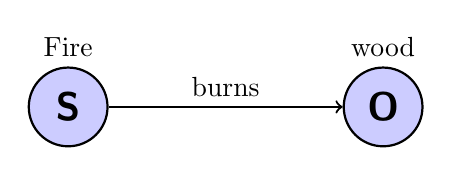
\begin{tikzpicture}[auto,node distance=2cm,thick,main node/.style={circle,fill=blue!20,draw,font=\sffamily\Large\bfseries}, scale=2]
    \node[main node, label=Fire,minimum size=1cm] (A) at (0,0) {S};
    \node[main node, label=wood,minimum size=1cm ] (B) at (2,0) {O};

    \path [->] (A) edge node {burns} (B);
    \end{tikzpicture}
\end{minipage}
\vspace{0.3cm}\\
For each of the triple statements exists such graph relationship, and altogether they make up the \textbf{RDF} model. Statements inside the \textbf{RDF} model that refer to the same subject or object are connected and form a semantic network.
\vspace{0.3cm}\\
When represented textually, for example in XML, the different components of a graph statement can come in different forms. A subject can be either a URI reference or a blank node, an object can be either a URI reference, blank node or a literal and a predicate can exist only as URI reference.\footnotemark[4] A \textbf{Uniform Resource Identifier reference}, often shortened to \textbf{URI ref}, is a Unicode string that only is made up from characters out of the ASCII Alphabet\footnote[5]{https://www.ietf.org/rfc/rfc2396.txt}. It is constructed out of five elements: \textcolor{red}{scheme}, \textcolor{blue}{authority}, \textcolor{green}{path}, \textcolor{orange}{query} and \textcolor{purple}{fragment}.\\ Altogether, the generic URI syntax looks like this:
\begin{center}
    \textcolor{red}{foo}\textcolor{blue}{://example.com:8042}\textcolor{green}{/over/there}\textcolor{orange}{?name=ferret}\textcolor{purple}{\#nose}\footnote[6]{Example taken from: https://en.wikipedia.org/wiki/Uniform\_Resource\_Identifier}
\end{center}
This shows the similarity to the more popular \textbf{URL}, which is special case of an URI.
A \textbf{blank node} is a node that is neither a URI ref nor a literal, that's why it is also called an anonymous resource. A \textbf{literal} is used to represent  values such as numbers, text strings or dates.
\begin{center}
    \begin{figure}
        \centering
        \begin{tikzpicture}[auto,node distance=2cm,thick,main node/.style={circle,fill=blue!20,draw,font=\sffamily\Large\bfseries}, scale=2]
        \node[main node, label=Fire, minimum size=1cm] (A) at (0,0) {S};
        \node[main node, label=wood, minimum size=1cm] (B) at (2,0) {O};
        \node[main node, label=paper, inimum size=1cm] (C) at (0,1) {S}
        
        \path [->] (A) edge node {burns} (B);
        %\path [->] (C) edge node {is made out of} (B);
        \end{tikzpicture}
        \caption{An example of a simplified RDF Model}
    \end{figure}
\end{center}

\section{RDFLib}
\section{D2RQ platform}
\subsection{D2R-server}
\subsection{D2RQ mapping language}

\chapter{Assignment and results}
\section{Current state of the pipeline}
\section{Implementation of the revised version}
\section{Results}
\section{Comparison to the previous pipeline}

\chapter{Conclusion and outlook}
\chapter{List of figures}
\chapter{Literature}

\appendix
\printbibliography
\end{document}
